\chapter{Sistemes guiats amb simetria translacional}

\section{Introducció}

Una guia d' ona és una estructura que restringeix l' expansió d' una ona a una regió de l' espai, de manera que aquesta és propaga desde la font fins a un lloc desitjat minimitzant la pèrdua d' energia. En general consisteixen en una capa de material conductor que envolta la regió de propagació, com a la figura \cref{fig:waveguide}.

\begin{figure}[ht]
  \centering
  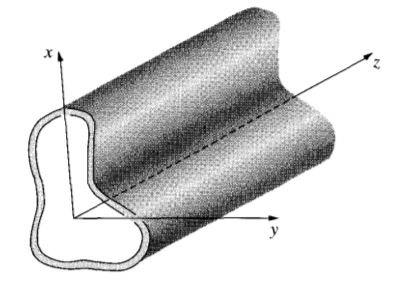
\includegraphics[scale=0.4]{arbitrary}
  \caption{Guia d' ona amb simetria translacional}
  \label{fig:waveguide}
\end{figure}

\section{Ones electromagnètiques}

Per a estudiar el comportament del camp electromagnètic en presència de conductors necessitem resoldre les equacions de Maxwell en zones sense càrrega (i.e. $\rho = \vec J = 0 $) junt a les condicions de contorn imposades pel sistema. 

\begin{subequations}
  \begin{align}
     \del \rfield D &= 0, \label{ME1}\\
     \curl \rfield E &= - \pd{\rfield B}{t}, \label{ME2}\\
     \del \rfield B &=0,  \label{ME3}\\
     \curl \rfield H &= \pd{\rfield D}{t} \label{ME4}
  \end{align}
\end{subequations}

Açò es simplifica als sistemes amb simetria translacional, en que les propietats dels material són constants al llarg d' una direcció espacial. Com que les propietats dels materials seran constants suposarem també que el perfil temporal del camp, que depén sobretot de la font, es manté amb el temps, i que aquest perfil és harmònic amb el temps, de manera que podem separar els camps en dos components (en general treballarem amb camps imaginaris, entenent que en realitat el camp és sols la part real):

\begin{subequations}
  \begin{align}
    \rfield E \rtfun = E\rfun\e{\jmath \omega t} \label{harmE}\\
    \rfield H \rtfun = H\rfun\e{\jmath \omega t} \label{harmH}
  \end{align}
\end{subequations}

Aquesta suposició simplifica enormement les matemàtiques, i en casos en que la font no és harmònica  podem utilitzar anàlisi de Fourier i descomposar-la en components que si ho són. La majoria de les fonts, de qualsevol manera, són d' aquest tipus.

Si substituim \cref{harmE,,harmH} en \cref{ME1,ME2,ME3,ME4} obtenim equacions de Helmholtz \footnote{Sempre i quan el medi siga lineal, isòtop i homogeni, cosa que suposarem durant tot el curs. També donarem per sentat que el medi no és magnètic, pel que $\mu{}_r  \sim 1$.}:

\begin{subequations}
    \label{helm}
  \begin{align}
    \del ^2 \vec E + k^2 \vec E &= 0 \\
    \del ^2 \vec H + k^2 \vec H &= 0 
  \end{align}
\end{subequations}

on $k = \omega \sqrt{\epsilon \mu} \nonumber$. Tenim ara sis equacions per a les components dels camps que podem resoldre per separació de variables. Resoldrem sols el cas $E_x$, ja que la resta són anàlegs:

\begin{equation}
  \label{eqdiffex}
  \pd[2]{E_x}{2} + \pd[2]{E_x}{t} + \pd[2]{E_x}{t} + k^2 E_x = 0
\end{equation}

Suposem $E_x \rfun = e_1(x)e_2(y)e_3(z)$, i com que $z$ és privilegiada (el material és simètric en aquesta direcció), fem $ E_x \rfun = f_t(x, y) f_z(z)$. Pel procediment habitual convertim \cref{eqdiffex} en dues noves:

\begin{equation}
  \frac{1}{f_z}\pd[2]{f_z}{t} = - \beta ^2
\end{equation}

\begin{equation}
  \frac{1}{f_t} \left(\pd[2]{f_t}{x} + \pd[2]{f_t}{y} \right ) + k^2 = \beta ^2
\end{equation}

On $\beta$ és un paràmetre independent que desconeixem. El signe i el quadrat han sigut introduïts per conveniència.

La solució de la primera és $f_z(z) \propto \e{ \pm \jmath \omega t}$. La segona és un altra equació de Helmholtz que deixem sense resoldre:

\begin{equation}
  \pd[2]{f_t}{x} + \pd[2]{f_t}{y}  + (k^2 - \beta ^2) f_t = 0
\end{equation}

Fent el mateix amb les altres 5 equacions obtenim camps harmònics en $z$ amb freqüència espacial $\beta$:

\begin{align}
  \rfield E \rtfun = ( \vec{e_t} + \vec e_z ) \e{\jmath(\omega t - \beta z)}  \\
  \rfield H \rtfun = ( \vec{h_t} + \vec h_z ) \e{\jmath(\omega t - \beta z)}
\end{align}

En principi tenim sis equacions, però podem reduir-les a dues si utilitzem les equacions de Maxwell sobre els camps. Usarem l' operador $\del$ descompost:

\begin{equation}
  \del = \pd{\,}{x}\ux + \pd{\,}{y}\uy +\pd{\,}{z}\uz = \del _t - \jmath \beta \vec u_z
\end{equation}

La component $z$ és queda així perquè anem a aplicar l' operador sobre camps harmònics en $z$, pel que $\pd{}{z}$ té el mateix efecte que multiplicar per $-\jmath \beta$.

Aplicant la llei de Faraday \cref{ME2} a aquests camps obtenim

\begin{equation}
  (\del_t-\jmath\beta\uz)\times (\vec e_t +\vec e_z) = -\jmath\omega\mu (\vec h _t + \vec h_z) 
\end{equation}

Separant els resultats en components $z$ i $T$:

\begin{equation}
  \del _t \times \vec e_t = -\jmath \omega\mu(\vec h_z ) \label{eT}
\end{equation}

\begin{equation}
  -\uz \times (\del _t \vec e_z ) -\jmath \omega \times \vec e_t = -\jmath \omega \mu \vec h _t \label{eZ}
\end{equation}

Fent el mateix amb la llei d' Ampère \cref{ME4} s' obté:

\begin{equation}
  \del _t \times \vec h_t = \jmath \omega\epsilon(\vec e_z) \label{hT}
\end{equation}

\begin{equation}
  -\uz \times (\del _t \vec h_z ) -\jmath \omega \times \vec h_t = -\jmath \omega \epsilon \vec e _t \label{hZ}
\end{equation}

Si $e_z = h_z = 0$ tenim que $\del_t \times e_t = \del_t \times h_t = 0$ existeixen potencials escalars i vectorials i el problema és redueix a resoldre les equacions de Laplace per a aquests. En cas contrari podem aïllar $\vec h_t $ en \cref{eZ} i $\vec e_t$ en \cref{hZ} i substituir en \cref{eT} i \cref{hT}, per obtindre les expressions:

\begin{equation}
  \label{soleT}
  \vec e_t = \frac{\jmath}{\beta ^2 - \omega ^2 \mu\epsilon} (\beta \del _t \vec e_z + \omega \mu \del _t \times \vec h_z )
\end{equation}

\begin{equation}
  \label{solhT}
  \vec h_t = \frac{\jmath}{\beta ^2 - \omega ^2 \mu\epsilon} (\beta \del _t \vec h_z - \omega \epsilon \del _t \times \vec e_z )
\end{equation}

Si usem aquestes expressions en \cref{eT} i \cref{hT} junt a l' identitat $\del \times (\curl \vec A ) = \del (\del \cdot \vec A) - \del ^2 \vec A$ i \cref{ME1,ME3} arribem a dues equacions de Helmholtz per als components en $z$:

\begin{equation}
  \label{helmhz}
  \del ^2 h_z + (k^2 - \beta ^2) h_z = 0
\end{equation}

\begin{equation}
  \label{helmez}
  \del ^2 e_z - (k^2 - \beta ^2) e_z = 0
\end{equation}

Per a calcular $\rfield E$ i $\rfield H$ en tot l' espai, per tant, hem de resoldre aquestes equacions junt a les condicions de contorn apropiades i obtindre $e_z$, $h_z$ i $\beta$, dels quals podem obtindre $\vec e_t$ i $\vec h_t$.

\section{Espectre mode i propietats de tall}

\subsection{Modes TEM}

Si $e_Z = h_Z = 0 $ les solucions per als camps s' anomenen modes TEM (transversal electromagnètic) i són particularment simples. De \cref{eT,hT} tenim que $\del_t \times \vec e_t = \del_t \times \vec h_t = 0$, i com hem dit abans podem utilitzar mètodes d' electrostàtica per a obtindre els components transversals. De \cref{eZ,hZ} tenim que

\begin{figure}[ht]
  \centering
  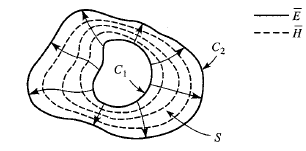
\includegraphics[scale=0.5]{arbitraryTEM}
  \caption{Mode TEM en una guia arbitraria}
  \vspace{-1 em}
\end{figure}

\begin{subequations}
  \begin{align}
    -\jmath \beta \uz \times \vec e_t &= -\jmath \omega \mu \vec h_t \\
    -\jmath \beta \uz \times \vec h_t &=  \jmath \omega \epsilon \vec e_t  
  \end{align}
\end{subequations}

Aïllant $\vec h_t$ en la primera equació i substituint en la segona arribem a $\beta = \omega \sqrt{\mu \epsilon}$. En el mode TEM, per tant, les ones de la guia és comporten com a ones planes, i els camps elèctric i magnètic estan relacionats per

\begin{equation}
  \vec h_t = \frac{\epsilon}{\mu} \uz \times \vec e_t = Y_{TEM} \uz \times \vec e_z
\end{equation}

On $Y_{TEM}$ és l' admitància del mode TEM en la guía.

\subsection{Modes TE}

Quan $e_z = 0$ però $h_z \neq 0$ les solucions s' anomenen modes TE (transversal elèctric). De \cref{soleT,solhT} obtenim que 

\begin{equation}
  \vec e_t = - \frac{j\omega\mu}{k_c^2} \del_t \times \vec h_z
\end{equation}

\begin{equation}
  \vec h_t = - \frac{\jmath\beta}{k_c^2} \del_t \times \vec h_z
\end{equation}

On hem definit $k_c ^2 = \omega^2 \mu\epsilon - \beta^2$. D' ací podem arribar a la relació

\begin{equation}
  \vec e_t = -Z_{TE} \uz \times \vec h_z
\end{equation}

On $Z_{TE} = \frac{\omega \mu}{\beta}$ és la impedància de la guia. Per a obtindre els camps, per tant, sols cal calcular $h_z$ i $\beta$ amb la equació de Helmholtz \cref{helmhz} i usar el resultat per a obtindre $\vec h_t$ i $\vec e_t$

\subsection{Modes TM}

Per un procediment anàleg podem obtindre els camps en el cas TM (transversal magnètic), en que $h_z = 0$ però $e_z \neq 0$.

\subsection{Modes híbrids}

Als modes híbrids, en que $e_z \neq 0$ i $h_z \neq 0$ cal resoldre les equacions de Helmholtz \cref{helmez,helmhz} i usar \cref{soleT,solhT} per a obtindre tots els camps.

\subsection{Propietats de tall}

Fins ara hem assumit que $\beta$ és real, però també pot ser imaginari, depenent de la freqüència de la ona i de $k_c$, ja que $\beta = \sqrt{\omega ^2 \mu\epsilon - k_c^2}$. Si $\omega ^2 \mu\epsilon > k_c^2$ tindrem $\beta$, i el factor $\e{\jmath(\omega t - \beta z)}$ és harmònic, però si $\omega ^2 \mu\epsilon < k_c^2$ tindrem $\beta$ imaginari, i $\e{\jmath(\omega t - \beta z)} = \e{-\vert\beta\vert z} \e{\jmath\omega t}$, pel que la ona s' atenuarà sense propagar-se, i diem que el mode està tallat (encara que no significa que no siga útil). La freqüència de tall (la mínima que ha de tindre una ona per a propagar-se) és, per tant, $\omega_c = k_c \sqrt{\mu\epsilon}$. Per als modes TEM, en que $k_c = 0$, $\omega_c = 0$, i els modes sempre es propaguen.

\section{Diagrama $\omega - \beta$ i dispersió}

La relació entre $\beta$ i $\omega$ ens dona la capaticat de propagació de la guia per a la ona. En un mode TEM seran proporcionals; en qualsevol altre mode la relació serà un poc més complicada. A més de determinar si la ona és propaga o no, també ens determina a quina velocitat ho fa: anomenem velocitat de fase a la quantitat $v_f = \frac{\omega}{\beta}$, i velocitat de grup a $v_G = \frac{d\omega}{d\beta{}}$. En el mode TEM són $0$ i $c$, respectivament, i a la resta de casos dependràn de $\beta(\omega)$.

\subsection{Velocitat de fase}

La fase de tots els components de $\rfield E$ i $\rfield H$ és $\e{\jmath(\omega t - \beta z}$. Com avancen els punts de la ona que tenen la mateixa fase? Si fem $d(fase) = 0$ obtenim $\omega dt - \beta dz = 0$, d' on $\frac{dz}{dt} = \frac{\omega}{\beta} = v_f$.

\subsection{Velocitat de grup}

Suposem que injectem una ona de freqüència pura  $\vec E_{in} \rtfun = \vec E_0  \e{\jmath \omega_0 t}$ en una guia, i obtenim a l' altre extrem $\vec E_{out} \rtfun = \vec E_0 \e{\jmath(\omega_0 t \beta \vert_{\omega _o} z)}$.  L' anàlisi freüèncial ens dona el mateix resultat: la transformada de Fourier de $\vec E_{in}$ és

\begin{equation}
  \hat E_{in} (\omega) = \frac{1}{2\pi} \int E_0 \e{\jmath\omega_0 t} \e{-\jmath \omega t} dt = E_0 \delta (\omega - \omega_o)
\end{equation}

ja que és una freqüència pura, i per tant la ona resultant és

\begin{equation} 
  \vec E_{out} \rtfun = 
  \int \hat E_{in} (\omega) \e{\jmath(\omega t - \beta \vert_{\omega _0} z)} dz =  
  \int \hat E_{o} \delta (\omega - \omega _0) \e{\jmath(\omega t - \beta \vert_{\omega _0} z)} dz = 
  E_0 \e{\jmath(\omega_0 t - \beta \vert_{\omega _0} z)} 
\end{equation}

Si en canvi transmitim un conjunt de freqüències simultàniament, per exemple per a transmetre una portadora modulada amb una senyal $I(t)$, bé amb modulació per fase, freqüència o ampitud, la ona entrant és $E(z=0) = I(t) \e{\jmath \omega _0 t}$, i veguem que ara $\vec E _{out} \neq I(t) \e{\jmath(\omega_0 t - \beta  \vert_{\omega _0} z)}$, perquè cada component $\omega$ es comportarà d' una manera diferent, com anem a vore. Si la TdF de $I(t)$ és $\hat I(\omega)$ la de $I(t)\e{\jmath \omega _0 t} $ és $\hat I(\omega - \omega _0)$, i per tant

\begin{equation}
  \hat E(z = 0, \omega ) = \frac{1}{2\pi} \int I(t) \e{\jmath\omega_0 t} \e{-\jmath\omega t} dt = \hat I(\omega - \omega _0)
\end{equation}

i la ona propagada resultant será una deformació de la ona inicial:

\begin{equation}
  E(z, t) = \int \hat E(z = 0, \omega) \e{\jmath(\omega t - \beta z)} d\omega = \int \hat I (\omega - \omega _0)  \e{\jmath(\omega t - \beta z)} d\omega
\end{equation}

En el cas en que l' ample de banda $\Delta \omega = \omega - \omega_0$ és xicotet podem expandir $\beta(\omega) = \beta ( \omega _0 ) + \left. \frac{d \beta}{d\omega}  \right\vert_{\omega _0} (\omega - \omega_0)$ i la integral té solució anal·lítica:

\begin{equation}
  E(z, t) = 
  \int \hat I ( \omega - \omega _0) \exp{ \jmath \left(\omega t + \left [\beta(\omega_0) + \left.\frac{d \beta}{d\omega} \right\vert_{\omega _0} (\omega - \omega_0) \right]z \right) }d\omega
\end{equation}

Fent un canvi de variable $ \omega \to \omega ' = \omega - \omega _0$ arribem a

\begin{equation}
  E(z, t) = I\left(t - \left. \frac{d\beta}{d \omega} \right \vert _{\omega _0} z\right) \e{\jmath(\omega_0 t - \beta(\omega _0) z )} 
\end{equation}

On s' aprecia que la ona entrant s' ha propagat amb un retrás $\tau = \left. \frac{d\beta}{d \omega} \right \vert _{\omega _0} z$, i podem definit la velocitat de grup $v_g = \frac{z}{\tau} = \frac{1}{\left. \frac{d\beta}{d \omega} \right \vert _{\omega _0} }$

\section{Potència transmessa per mode}

Una vegada hem calculat els camps corresponents a un mode, podem clacular la potència que transmet aquest per la guia usant el teorema de Poynting.

\begin{equation}
  \mathcal P = \frac{1}{2} \int \rfield E \times \rfield H \cdot d \vec S = \frac{1}{2} \int \rfield E \times \rfield H \cdot (dS \uz) = \frac{1}{2} \int \vec e_t \times \vec h_t  \cdot (dS \uz)
\end{equation}

\section{Pèrdues d' energia}

Assumirem que la potència perduda per unitat de longitud és proporcional a la potència que flueix pel sistema, ja que el nombre de fonons en el material será propocional al nombre de fotons transmesos.

\begin{equation}
  \frac{dP}{dz} = -\alpha P \to P = P_0 \e{- \alpha z}
\end{equation}

A la constant de proporcionalitat $\alpha$ l' anomenem factor d' atenuació.

\subsection{Atenuació per dielèctric}

Si el medi interior de la guia té un dielèctric l' ona perdrà amplitud al viatjar per ella. Les caracteritzarem amb una permeabilitat elèctrica complexa $\hat \epsilon = \epsilon' - \jmath \epsilon '' $, que en la llei d' Ampère dona lloc a una corrent de pèrdues:

\begin{equation}
  \curl \rfield H = \jmath \omega \hat \epsilon \rfield E = \jmath \omega \epsilon ' \rfield E + \omega \epsilon '' \rfield E = \jmath \omega \epsilon ' \rfield E + \sigma _c \rfield E = \jmath \omega \epsilon ' + \rfield J _p
\end{equation}

L velocitat de propagació també és vorà afectada:

\begin{equation}
  \hat \beta = \sqrt{\omega ^2 \mu\hat \epsilon } = \sqrt{\omega^2 \mu\epsilon'-\omega^2 \mu\epsilon '' \jmath - k_c ^2}
\end{equation}

Si les pèrdues són poques $\epsilon '' << \epsilon '$, i podrem aproximar

\begin{align}
  \hat \beta &\simeq  \sqrt{\omega^2 \mu\epsilon' - k_c} - j \frac{1}{2}\frac{\omega ^2 \mu\epsilon}{\sqrt{\omega ^2 \mu\epsilon ' - k_c ^2 }} \frac{\epsilon ''}{\epsilon '} \\ &= \beta - \jmath \frac{1}{2}\frac{\omega^2 \mu\epsilon}{\beta} \frac{\epsilon ''}{\epsilon'} 
= \beta -\jmath \frac{1}{2} \frac{k^2}{\beta }\tan \delta \nonumber 
\end{align}

El factor $\tan \delta$ s' anomena tangent de pèrdues, i depén solament del material.

\subsection{Pèrdues en conductors}

Als conductors sempre hi apareixerà una corrent de pèrdues associada al camp elèctric de la ona, que degut a la alta conductivitat $\sigma_c$ dominará la llei d' Ampère:

\begin{align}
  \curl \rfield H &= j \omega \epsilon \rfield E + \rfield J = \jmath \omega \epsilon \rfield E + \sigma _c \rfield E \\
 &\simeq \sigma _c \rfield E =  \jmath \omega \frac{\sigma _c}{\jmath \omega} \rfield E = \jmath \omega \hat \epsilon \rfield E \quad \text{amb} \quad \hat \epsilon = -\jmath \frac{\sigma _c }{\omega} \nonumber
\end{align}

La velocitat de propagació, com abans, serà afectada:

\begin{equation}
  \hat \beta = \sqrt{-\jmath\omega \mu\sigma_c - k_c ^2} \simeq \frac{1-\jmath}{\sqrt 2} \sqrt{\omega \mu \sigma _c }
\end{equation}

El factor $\e{\jmath \omega t}\e{-\jmath \beta z} $ es convertirà en una atenuació:

\begin{equation}
  \e{\jmath \omega t} \e{ -\sqrt{\frac{\omega \sigma_c \mu}{2}} z} \e{-\jmath \sqrt{\frac{\omega \sigma_c \mu}{2}} z}  = \e{\jmath \omega t} \e{- \frac{z}{\Delta}} \e{-\jmath \frac{z}{\Delta}}
\end{equation}

on $ \Delta = \sqrt{\frac{2}{\omega \sigma _c \mu}}$ és la profunditat de penetració. En materials molt conductius, com els metalls, aquesta distància serà molt curta, normalment una micra o dos, en la qual la potència dissipada per els camps al conductor serà

\begin{align}
  \mathcal P _l &= \frac{1}{2} \int \rfield E \rfield J ^* dV = \frac{1}{2} \int \rfield J \sigma _c \rfield J^* dV = \frac{\sigma _c }{2} \int \left \vert \curl \rfield H \right \vert ^2 dV \\
  &= \frac{\sigma _c}{2} \left \vert \frac{1 + \jmath}{\Delta} \right \vert ^2 \int \left \vert \rfield H _{sup} \right \vert ^2 \left \vert e ^{- \frac{z}{\Delta}} e ^{-j \frac{z}{\Delta}} \right \vert ^2 dV = \frac{\sigma_c}{2} \int _{z = 0} ^ {z = \infty} \left \vert H_{sup} \right \vert ^2 \e{-\frac{2z}{\Delta}} dS dz \nonumber \\
 &= \frac{1}{2} \sqrt{\frac{\omega \mu}{2\sigma _c}} \int _{superficie} \left \vert H_{sup} \right \vert ^2 dS= \frac{\mathcal {R _s}}{2} \int _{superficie} \left \vert H_{sup} \right \vert ^2 dS \nonumber 
\end{align}

El terme $\mathcal R_s$ s' anomena resistència superficial del metall, i és interesant observar que la forma final de $\mathcal P$ recorda a la dels circuits $P = R I ^2$.

\section{Decibels}

De vegades usarem decibels per a expressar atenuacions (o guanys) de potència. Si la potència d' entrada $P_0$ s' ha atenuat (o amplificat) fins a $P$ el factor $\alpha$ en decibels és

\begin{equation}
  \alpha_{dB} = 10 \log_{10} \frac{P}{P_0}
\end{equation}

(si $P < P_0$ el resultat serà negatiu, i viceversa). La utilitat d' aquesta definició és que per a obtindre l' atenuació (o guany) total produïda per factors multiplicatius (per exemple en una sèrie de components) podem simplement sumar els decibels de cada factor.

Quan la quantitat d' interés és proporcional a $P^2$, com $\abs{E_0}$ o $V$, l' exponent ix fora i queda 

\begin{equation}
  \alpha_{dB} = 20 \log_{10} \frac{E}{E_0}
\end{equation}